% options:
% thesis=B bachelor's thesis
% thesis=M master's thesis
% czech thesis in Czech language
% english thesis in English language
% hidelinks remove colour boxes around hyperlinks

\documentclass[thesis=B,english]{FITthesis}[2012/10/20]

\usepackage[utf8]{inputenc} % LaTeX source encoded as UTF-8
% \usepackage[latin2]{inputenc} % LaTeX source encoded as ISO-8859-2
% \usepackage[cp1250]{inputenc} % LaTeX source encoded as Windows-1250

\usepackage{graphicx}
 %graphics files inclusion
% \usepackage{subfig} %subfigures
\usepackage{amsmath} %advanced maths
\usepackage{amssymb} %additional math symbols
% \usepackage{algpseudocode}
% \usepackage{algorithm}
% \usepackage{algorithmicx}
\usepackage{listings}
\lstdefinelanguage{JavaScript}{
  keywords={break, case, catch, continue, debugger, default, delete, do, else, finally, for, function, if, in, instanceof, new, return, switch, this, throw, try, typeof, var, void, while, with},
  morecomment=[l]{//},
  morecomment=[s]{/*}{*/},
  morestring=[b]',
  morestring=[b]",
  sensitive=true
}
\usepackage[ruled,vlined,linesnumbered]{algorithm2e}
\usepackage{dirtree} %directory tree visualisation
% % list of acronyms
\usepackage[acronym,nonumberlist,toc,numberedsection=autolabel]{glossaries}
% \iflanguage{czech}{\renewcommand*{\acronymname}{Seznam pou{\v z}it{\' y}ch zkratek}}{}
\makeglossaries

\newcounter{eqn}
\renewcommand*{\theeqn}{\alph{eqn})}
\newcommand{\num}{\refstepcounter{eqn}\text{\theeqn}\;}

\makeatletter
\newcommand{\putindeepbox}[2][0.7\baselineskip]{{%
    \setbox0=\hbox{#2}%
    \setbox0=\vbox{\noindent\hsize=\wd0\unhbox0}
    \@tempdima=\dp0
    \advance\@tempdima by \ht0
    \advance\@tempdima by -#1\relax
    \dp0=\@tempdima
    \ht0=#1\relax
    \box0
}}
\makeatother


% % % % % % % % % % % % % % % % % % % % % % % % % % % % % % 
% EDIT THIS
% % % % % % % % % % % % % % % % % % % % % % % % % % % % % % 

\department{Department of Computer Science}
\title{Application of Random Decision Forests in Astroinformatics}
\authorGN{Andrej} %author's given name/names
\authorFN{Pali{\v c}ka} %author's surname
\author{Andrej Pali{\v c}ka} %author's name without academic degrees
\authorWithDegrees{Andrej Pali{\v c}ka} %author's name with academic degrees
\supervisor{RNDr. Petr {\v S}koda, CSc.}
\acknowledgements{I would like to thank my supervisor, RNDr. Petr {\v S}koda, CSc., for his help and insight.}
\abstractEN{In this bachelor's thesis we examine a machine learning model called the Random Decision Forest and its performance on astronomical problems. We present an overview of existing implementations and algorithms that are suitable for Big Data. We wrapped several implementations of RDF into one package that can be run with a single command. We conducted experiments on both classification and regression problems and compared the results with other data mining algorithms. The experiments were performed on some well known data sets from the UCI repository and on some astrophysical problems, particularly spectra classification. The outcomes of the experiments show very promising results.}
\abstractCS{V tejto bakalárskej práci sme skúmali algoritmus strojového učenia zvaný náhodné rozhodovacie lesy (Random Decision Forest) a jeho účinnosť na astronomických dátach. Ukážeme prehľad existujúcich imeplementácii a algoritmov, ktoré sa hodia na veľké dáta. Implementovali sme aplikáciu, ktorá zabalila niekoľko implementáci RF do jedného balíku a z ktorého sa môžu spúšťať jedným príkazom. Experimentovali sme na klasifikačných aj regresných problémoch a porovnali sme výsledky týchto experimentov s ďalšími algoritmami strojového učenia. Tieto experimenty sme vykonali ako na známych dátach z UCI repozitória, tak na astronomických problémoch, špeciálne na klasifikácii spektier. Výsledky týchto experimentov sú veľmi prespektívne.}
\placeForDeclarationOfAuthenticity{Prague}
\keywordsCS{rozhodovacie stromy, rozhodovacie lesy, vyťažovanie znalostí z dát, astroinformatika}
\keywordsEN{decision trees, decision forests, data mining, astroinformatics}
\declarationOfAuthenticityOption{4} %select as appropriate, according to the desired license


\begin{document}

\newacronym{CVUT}{{\v C}VUT}{{\v C}esk{\' e} vysok{\' e} u{\v c}en{\' i} technick{\' e} v Praze}
\newacronym{FIT}{FIT}{Fakulta informa{\v c}n{\' i}ch technologi{\' i}}

\setsecnumdepth{part}
\chapter{Introduction}
Machine learning has become a phenomenon in recent years. Many businesses, institutes or organizations are increasingly more dependent on getting knowledge from data they managed to gather through their endeavors. One field that could highly benefit from machine learning is astroinformatics.  Astronomical surveys generate terabytes of data during one session. This amount of data requires an unconventional approach in terms of storage, analysis and evaluation.  

Random Decision Forest \cite{BR01} is an ensemble model that has proven to be successful on data, that contain large amount of features and instances. In this thesis we attempt to describe this model and its properties. We also make a survey of some of the available RDF algorithms and implementations, with regard to their performance on big data. We will implement a package, that wraps around several RDF implementations. We will perform tests both on data sets in the UCI repository \cite{uci} and on astronomical data.

We introduce common data mining and machine learning concepts and techniques in chapter~\ref{chap:DM}. Chapter~\ref{chap:DT} discusses the basic block of the RDF: the Decision Trees. Since some distributed RDF algorithms require parallel tree building process we also examine some scalable approaches to the induction of Decision Trees. Chapter~\ref{chap:RDF} defines the RDF, examines some of their properties, and provides examples of both serial and parallel implementations of the algorithm. We implement a wrapper that binds several RDF implementations together and we describe it in chapter~\ref{chap:wrapper}. In chapter~\ref{chap:Experiments} we show results from our experiments with the Random Decision Forest model on astronomical data as well as on some common data sets.
\setsecnumdepth{all}

\chapter{Knowledge discovery, data mining and astroinformatics}
\label{chap:DM}
Knowledge discovery from databases (KDD) is an interactive and iterative ``process of identifying valid, novel, potentially useful, and ultimately understandable patterns in data'' \cite{andrassyova1999knowledge,Fayyad96thekdd}. Data mining (DM) is usually defined as a process where ``intelligent methods are applied to extract data patterns'' \cite{han2006data} and is merely a step in the process of KDD, however these two terms are often used synonymically. The KDD consists of these steps \cite{han2006data}:
\begin{description}
	\item[Data cleaning:] removing noise and incorrect data
	\item[Data integration:] combination of different data sources
	\item[Data selection:] selection of relevant data
	\item[Data transformation:] transformation of data into a format that is suitable for data mining
	\item[Data mining:] applying DM algorithms
	\item[Pattern evaluation:] evaluating the patterns that the DM process extracted and selecting those, that are relevant for our goal
	\item[Knowledge presentation:] transforming of extracted knowledge into a form that a user can understand
\end{description}

Data mining process involves building models based on some data. These models then help to extract patterns and relationships that are hidden inside the data. DM algorithms consist of a mix of three components \cite{Fayyad96thekdd}:
\begin{description}
\item [The model:] The model consists of a function and a representational form. The function determines what the model will do, e.g. classification or regression. The representational form means how the model will represent the data, e.g. a decision tree or a density function. The model contains parameters that are determined from the data.
\item [The preference criterion:] it computes a quality of model and helps to choose the model over others. It is usually a goodness-of-fit function of the model to the data.
\item [The search algorithm:] The function used when the model is constructed and fitted to the data.
\end{description}

This thesis concerns itself with a model that is represented in the form of a decision forest with a function capable of both classification and regression. The search algorithms are from a family of heuristic functions and a preference criterion is a generalization error.

\section{Data mining methods}
A machine learning algorithm tries to learn a certain function that either describes the data in some way, or tries to predict an outcome. We recognize these basic methods of data mining \cite{fayyad1996data}:
\begin{description}
\item [Classification] This method maps the data set to a known finite set containing the labels. An example of classification is a model that decides whether a certain email message is a spam or not.
\item [Regression:] This method tries to predict a value of some numeric variable. An example of a regression may be prediction of redshifts based from the spectra.
\item [Clustering:] This method describes the data and tries to find a previously unknown finite set of categories the data would fall in. These categories can overlap each other, if certain data belong to multiple categories. An example of clustering may be discovering kinds of stars from spectra.
\item [Summarization:] This method attempts to find a compact description of data. It may simply mean calculating some statistical properties like means for each field, or it could mean something more complex, like discovering functional relationships between attributes.
\item [Dependency modeling:] This method tries to find dependencies between variables. 
\item [Change and deviation detection:] This method detects data, that are in some way different than previously measured data. This includes finding outliers, which are data that are in some way different from the majority. It is useful for finding data that are worthy of further examination.
\end{description}

A learning can either be supervised or unsupervised. A supervised learning means that we have a training data set, where the relationships between variables and their outcomes are already known. These data sets usually come either from historical data (such as weather patterns), or were labeled by humans specifically for the purpose of serving as a testing set. This can however bring bias and noise to the set. An unsupervised learning means, that the model is built from the data, that were not evaluated by anyone and where the relationships are unknown. The model has to discover these relationships and their possible outcomes by itself.

\section{Data set}
A data set is a collection of data. It can take form of a CSV file, FITS file, image, sound wave, etc. Machine learning algorithms however usually work with a data set represented as a table, where each column represents a variable and each row represents a datum. A member of the data set is again a collection of values that represent its respective variable. A variable may be either categorical (discrete), or numerical (continuous).

\section{Model validation and scoring}
After a model is fitted over some data we have to determine how it will perform when used to analyze data it has not seen yet. This is usually done by splitting the original set into a separate testing and training set. We first train the model with the testing set and then assess its performance by running a test over the training set and comparing the results of the testing run with what the true results in the testing set. There are several scoring measures that estimate how well the model did on the testing set. A simple measure that can be used for classification would be one that computes a ratio of the correctly classified data out of all the data. A more advanced measure is for example the \(F_1\) measure, which defined as
\[
F_1=2*\frac{\textit{precision}*\textit{recall}}{\textit{precision}+\textit{recall}}
\]
where precision signifies the fraction of correctly identified objects out of all that were identified and the recall means fraction of correctly identified objects of one class out of all the objects of the class. However this measure can only be used in a binary classification. In case more than two classes are present, one has to perform this measure for each class separately by considering that particular class as class one and all the other classes as class two.

If the model performs a regression, however, it has to use a different metric. A mean squared error is usually used.
\section{Astroinformatics}
Astroinformatics is a new discipline, that attempts to apply concepts from computer science and machine learning on astronomical problems. Modern astronomy now is producing terabytes or even petabytes of data \cite{borne2009scientific}, with more to come in the future. For example the LSST will, upon its completion, generate half a petabyte of data every month \cite{becla2006designing} that will require processing and analyzing.

\chapter{Decision trees}
\label{chap:DT}
		Decision trees are a group of supervised data mining methods, that use a tree-like structure to analyze data. They can perform either a classification of data, or a regression of data. The inner nodes of a decision tree represent testing on input attributes. \cite{CMP07} Terminal nodes in a classification tree represent the possible classes of tested objects. In a regression tree they represent predicted values for a given branch. Terminal nodes can either contain single values, or a probability vector of values \cite{TOP_DOWN_INDUCTION_SURVEY}. 

		The process of growing the decision tree is called an induction. Induction of an ideal decision tree is known to be NP-complete \cite{NP-COMPLETE}, so we have to use a heuristical approach for real-world applications. The induction consists of selecting the training data set, determining the splits at each nodes, choosing a stopping criterion and pruning of the tree. The methods we choose to perform these processes with directly affect the performance of the tree. 

		Traditionally \cite{CART,C45-NUMERICAL}, the induction of a DT is performed in a recursive fashion, which is fine for small data, but tends to fail on big data problems. Therefore algorithms that are designed for big data use breadth-first approach \cite{mehta1996sliq,ben2010streaming}.
		
		\section{Splitting the nodes}
			Splitting is generally the costliest and most important phase of the induction. For each internal node, the inductor examines the input attributes in attempt to find the best split, i.e. at least one attribute, upon which it would branch the node. 

			An attribute may be either categorical (discrete) or numerical (continuous). Evaluating categorical attributes is generally straightforward, the easiest solution is to just create a branch for each possible value. A more complex one is to group several values together and to create a branch for each value. We can use this to create binary decision trees.

			Additional steps must be taken when dealing with numerical attributes \cite{C45-NUMERICAL}.	 In this case the node is branched according to some threshold value or values which we need to find. At first, the data must be sorted based on the attribute. We'll mark those sorted values as \(\{v_1..v_m\}\). Each value \(v_i\) is then used as a discrete value by the splitting criteria to determine the best split between two values \(v_i\) and \(v_{i+1}\). Evaluating numerical attributes is much more costly that the evaluation of categorical attributes due to the need of sorting.

			To determine how to split the nodes in the tree, we need to evaluate splitting criteria. There are essentially two types of splitting criteria:
			\begin{itemize}
			\item Univariate
			\item Multivariate
			\end{itemize}
			The univariate splitting criteria split the node according to the value of one attribute, while the multivariate criteria split the node on multiple attributes.

			\subsection{Univariate criteria}
				There are several categories of univariate criteria, such as impurity-based, normalized impurity-based or binary criteria. \cite{DMWithDecisionTrees}
				\subsubsection*{Impurity-based criteria}
				Impurity-based criteria use an impurity measure, which is a function \(\phi\):\(\lbrack0,1\rbrack^k->R\). For an input feature \(X\) with \(k\) discrete values distributed with probability \(P=(p_1,\dots,p_k)\), \(\phi(P)\) satisfies the following conditions \cite{DMWithDecisionTrees}:
				\begin{enumerate}
				\item \(\phi(P) \geq 0\)
				\item It is minimum if \(\exists i\) such that \(p_i = 1\)
				\item It is maximum if \(\forall i, 1 \leq i \leq k, p_i = 1/k\)
				\item It is symmetric with respect to components of P.
				\item It is smooth (differentiable everywhere) in its range.	
				\end{enumerate}
				The goodness-of-split due to discrete attribute \(a_i\) is defined as reduction in impurity of the target attribute after partitioning \(S\) according to the values \(v_{i,j} \in \textit{dom}(a_i)\):
				\[
					\Delta\phi(a_i,S)=\phi(P_y(S))-\sum\limits_{j=1}^{|\textit{dom}(a_i)|}{\frac{|\sigma_{a_i}=v_{i,j}S|}{|S|}*\phi\left(P_y\left(\sigma_{a_i}=v_{i,j}S\right)\right)}
				\]

				\paragraph*{Information Gain}
				Information gain uses an entropy of the input attributes as the impurity measure. The entropy of a set D is defined as:
				\[
				\textit{Entropy}\left(y, S\right) = \sum _{c_j \in \textit{dom(y)}}-\frac{|\sigma_{y=c_j}S|}{|S|}*\log_2\frac{|\sigma_{y=c_j}S|}{|S|}
				\] 
				Because of the attributes of the entropy, it tends to favor attributes with a lot of values. This can turn out to be problematic, for example if we include attributes that are unique for each specimen, such as their ID \cite{ENSEMBLE}. This can be remedied by using a gain ratio instead. It normalizes the information gain against the number of values of the feature.
				\paragraph*{Gini index}
				The Gini index measures the divergences between the probability distributions of the target attributes values \cite{DMWithDecisionTrees}. It was popularized by the CART algorithm \cite{CART}. It is defined as follows:
				\[
					\textit{Gini}\left(y, S\right)=1 - \sum _{c_j \in \textit{dom(y)}}\left(\frac{|\sigma_{y=c_j}S|}{|S|}\right)^2
				\]
				\subsubsection*{Binary criteria}
				Binary criteria are used to create binary trees. Binary criteria divide the domain of the input attribute into two subdomains. Let \(\beta(a_i, d_1, d_2, S)\) be a binary criterion value for attribute \(a_i\) over the data set \(S\) that divides it into two mutually exclusive and exhaustive subdomains \(d_1\) and \(d_2\). The binary criterion attempts to find the maximum value for the split, while satisfying the conditions for \(d_1\) and \(d_2\). An example of binary criterion is a twoing criterion. It was suggested in \cite{CART} after discovering that the Gini index performs badly when encountering wide domains. The twoing criterion is defined as
				\begin{multline*}
					\textit{twoing}(a_i, S, d_1, d_2) = 0.25 * \frac{|\sigma_{a_{i} \in d_1}S|}{|S|}* \frac{|\sigma_{a_{i} \in d_2}S|}{|S|}  * \\ \left(\sum_{c_{1}\in\textit{dom}(y)}{
					\left|
					\frac{\left|
							\sigma_{a_{i}\in d_{1} \wedge y=c_i}S
						\right|}
						{|\sigma_{a_{i} \in d_1}S|} - \frac{\left|
							\sigma_{a_{i}\in d_{2} \wedge y=c_i}S
						\right|}
						{|\sigma_{a_{i} \in d_2}S|}
					\right|
					}\right)^2
				\end{multline*}
				\subsubsection*{Regression criteria}

				We have to use different criteria in regression, because we are dealing with continuous target values, instead of discrete. An example of criterion that is used for regression is minimization of a \textit{mean-square error}. It minimizes the square of the error between what is predicted and what should be the actual result. It is defined as:
				\[
					\textit{MSE}\left(y, \textit{pred}\right)= \frac{1}{|dom(y)|}*\sum _{c_j \in \textit{dom(y)}}\left(c_j - \textit{pred}\right)^2
				\]

		\subsection{Multivariate criteria}
			Although multivariate criteria are more effective than univariate, they are much more difficult to implement. They are usually based around finding the best linear combination of the attributes. Methods for finding this combination include:
			\begin{itemize}
				\item Neural trees \cite{NTrees}
				\item Hill climbing \cite{CART}
				\item Linear programming
			\end{itemize}

		\section{Stopping criteria and pruning}
			Stopping criteria tell the inducer when to stop splitting the nodes. Upon fulfilling the stopping criteria, the node is assigned the output label instead of splitting. There are various conditions and their combinations that can be used as the criteria, such as reaching the maximum tree depth, not gaining any significant information from the splitting criteria or not having enough cases in nodes. Choosing the right stopping criteria is vital for the tree, because choosing very strict criteria may lead to an underfit tree. Making the criteria too benevolent, however, leads to overfitting the tree and losing information about the relationship between various attributes. To provide a solution, \cite{CART} introduced a pruning algorithm, that allows the tree to overfit and then prunes it to remove branches that cause the tree to lose generality.
				
		\subsection{Pruning}
		\label{sec:pruning}
				\paragraph*{Cost-complexity pruning}

				This is a pruning method suggested by \cite{CART}. The pruning is executed in two phases. In the first phase, we produce a sequence of trees \(T_0, T_1, T_2, \dots, T_k \), were \(T_0\) is the initial unpruned tree obtained by the induction and \(T_k\) is a tree consisting only of the root node. Each tree is obtained by replacing one or more subtrees in its predecessor by leaves. To determine which subtree to remove, we calculate an increase in error rate per pruned leaf by 
				\[\alpha = \frac{\mathrm{err(pruned(}T,t\mathrm{)},S\mathrm{)} - \mathrm{err(}T,S\mathrm{)}}{|\mathrm{leaves(}T\mathrm{)}|-|\mathrm{leaves(}\mathrm{err(pruned(}T,t\mathrm{)}\mathrm{)}|}\]
				where \emph{err} is an error rate for given tree \(T\) and set \(S\), \emph{pruned} is a pruned tree from \(T\) without subtree \(t\) and \emph{leaves} is a number of leaves in \(T\).

				In the second phase, we compute the generalization error for each tree \(T_i\), and select the tree with the lowest error

				\paragraph*{Reduced-Error Pruning}

				This method was introduced by \cite{Quinlan1987221}. We perform a test run on the original tree and check for each non-leaf node, whether replacing it with the most common class would reduce the error rate. This process continues, until we cannot reduce the error rate any more.

		\section{Testing the data}
		Once the tree induction process is complete, we can begin with testing the unknown data. Beginning at the root node, each entry from the data is tested based on the attributes the node represents and then passed into the subtree, where the process repeats itself. Once it reaches the leaf node, it is assigned the outcome that is in the node. In case there is more than one outcome in the node, it is either chosen randomly, or with a probability determined by their distribution.
		
		\section{Decision trees algorithms}

			A general decision tree induction algorithm usually looks like this:

			\begin{algorithm}[H]
			\caption{BuildTree}
			\SetAlgoLined
			\KwData{
			\begin{itemize}
			\item data set $S$
			\item features vector $X$
			\item output class $Y$
			\end{itemize}
			}
			\KwOut{tree $T$}
			\Begin
			{
			\If{stopping criterion}{
				return
			}
			\ForEach{$x$ in $X$} {
				compute gain from splitting on $x$
				\If{computed gain is the largest so far} {
					save the attribute
				}
			}
			Split on the attribute with the largest gain \\
			Apply recursively on each node gained by the split \\
			return current node
			}
			\end{algorithm}

			\paragraph*{ID3} It is a very simple decision tree algorithm proposed by Quinlan in \cite{INDUCTIONOFDT}. It uses information gain as a splitting criterion. The induction stops either when all the data belong to a single value, or when the information gain is less than some threshold or equal to zero. The algorithm fails on missing attributes and cannot handle numerical attributes. It does not perform pruning.
			\paragraph*{C4.5} An improved version of the ID3 algorithm \cite{C45-NUMERICAL} that solves many of its problems. Instead of the information gain, it uses a gain ratio. The algorithm performs error-based pruning, handles missing values through corrected gain ratio criteria and can learn from data sets that contain numeric attributes. The growing can stop when the number of instances to be split is below certain threshold. Both ID3 and C4.5 cannot handle target labels that contain continuous values.
			\paragraph*{CART} Introduced in \cite{CART}. CART produces binary trees. What makes this algorithm significant and useful is that it handles both continuous and discrete output features and thus is capable of both classification and regression. It uses twoing criteria for classification and cost-complexity pruning. For regression it tries to minimize the prediction squared error. Users can enhance its accuracy by providing probability distribution \textit{a priori}, and it can consider missclassification cost.
			\subsection{Complexity analysis}
			We will examine the time complexity of a binary decision tree, using a univariate splitting criterion, that has been built on a data set of \(s\) samples with \(f\) features. During each step of the iteration, the tree has to evaluate each of the \(f\) features to find the best split. Assuming we presorted the feature lists before the induction and assuming on average balanced partitioning at each node, we have to search through \(f\log(s)\) samples at each node. Summing it over each node, we end up with complexity of \(\mathcal{O}(fs\log(s))\).
		\section{Performance and scalability}
		Traditional approaches to induction do not scale well for big data. Since they are usually built in a recursive fashion and require the data to be in the memory all the time, the system may run out of memory \cite{SCALABLE_RDF}. Another issue that has to be solved is the evaluation of attributes. As mentioned, the evaluation of numerical attributes is quite costly, because it involves sorting of all the values and then finding the best split. Many scalable algorithms try to speed up this process by pre-sorting the data \cite{mehta1996sliq,shafer1996sprint}, while others try to first pre-process them, as is the case with SPDT, which builds histograms from those attributes\cite{ben2010streaming}. Splitting on discrete attributes, while easier than splitting on numerical attributes, is not without its own problems. Search for a good split involves searching through subsets of the whole set of possible attributes, which in naive implementation would mean searching and selecting \(2^n\) possibilities, where \(n\) is the number of items in the set. Thus this also requires a quick algorithm \cite{mehta1996sliq}.

		To further overcome these limitations, we can parallelize the induction process, distributing it across several computing nodes. While this makes an implementation of the DT much more complicated, it allows for huge data sets, thus improving the accuracy of the tree.

		\subsection{Types of parallelism}
		There are several strategies for parallelization of DT using task parallelism, data parallelism or hybrid parallelism. \cite{PARALLEL_IMPLEMENTATION}
		\paragraph*{Task parallelism.} When using task parallelism, we distribute the decision nodes across several processors. The induction process starts on a single processor, which then proceeds with the induction as in the serial approach. When the number of decision nodes reaches the number of available processors, they are distributed among them. Then, each processor continues in the induction of the subtree with the assigned node as its root. The subtrees are then merged together as they are completed. An example of this approach is a parallel implementation of C4.5 algorithm in \cite{PARALLEL_INDUCTION}. 

		This approach has its disadvantages. The load on each processor is imbalanced, because each subtree can take considerably different time to construct. This could be countered by splitting the subtrees further, after some processor finished its task. Moreover, each processor needs to have access to the full data set, meaning it either has to be copied to each processor, or the processors have to access it from a central location, creating a great amount of communication. 

		\paragraph*{Data parallelism.} In data parallelism, the data, instead of the tree nodes, are split among the processors. The processors construct each node together, locally evaluating the data they were assigned. Because the processors have to communicate and share their split evaluations each time a new node is created the data parallelism generates a lot of communication on the network. The data can either be split vertically or horizontally. 

		In a vertical split, each processor receives every record and its label, but only a distinct set of input attributes. When deciding where to split, it takes into account only the set of attributes it received. Each processor supplies the best split from its local attributes. From these local splits the best one is picked. The vertical split strategy can still suffer from load imbalance, because continuous attributes usually take longer to evaluate.

		When using a horizontal split, each processor is assigned a distinct set of the records, but with full set of attributes. Each processor then examines possible splits based on the data it received and then communicates its findings with the other processors. They then work together to find the best global split.

		\paragraph*{Hybrid parallelism.} This is a combination of the data and task parallelism. It tries to combine the low communication overhead of the task parallelism with the lower memory requirements and processing amount of the data parallelism. The nodes that would have to cover large amount of examples use data parallelism to lower the load balance of each node. On the other hand, nodes, that cover few examples can be effectively distributed among several processors without significant memory overhead and thus eliminating costly interprocessor communication.

		\subsection{Streaming Parallel Decision Tree}
		Streaming Parallel Decision Tree (SPDT) is a state-of-the-art parallel Decision Tree algorithm. It can handle streaming data as well as traditional batch processing. It deals with large data sets by partitioning this data horizontally across several worker processors and building histograms out of them. The master processor then merges these histograms and uses them to find the best splitting point \cite{ben2010streaming}. 

		\section{Advantages and disadvantages}
		As we can see, one of the main advantages of a DT is its simplicity and intuitiveness. They can be used on all sorts of data, both for classification and for regression. They allow for errors in data and, with some improvements, can handle missing values well \cite{DMWithDecisionTrees,CMP07}. Decision trees can be converted to a set of rules just by following branches from the root node to a leaf node. Some are capable of handling both numeric and categorical values and some algorithms can be used both for classification and regression.

		On the other hand, non-parallel decision trees do not perform well on high dimensional data. They are also sensitive to noise and irrelevant attributes and they easily overfit or underfit.
\chapter{Random Decision Forests and Random Ferns}
\label{chap:RDF}
	RDF is an ensemble classification method using \(K\) decision tree classifiers \({h(x, \Phi_k), k = 1\dots K} \), where \(x\) is the input data and \({\Phi_k}\) are independent identically distributed random vectors \cite{SELECTION_OF_DT}. The random vector \(\Phi_k\) represents the randomness that is injected into each DT and its nature and content is dependent on a concrete use. The randomness is usually introduced by randomly sampling the subset of input features and/or by bagging. After finishing the run in each tree, they vote for the final result, which will be chosen as the final class that will be assigned to that data entry.

	As with the Decision Trees, the performance of the RDF is directly affected by several factors such as the number of the trees, the means of introducing randomness into the induction, the voting process or the induction of the trees themselves.

	\section{Number of trees and their diversity}
	It can be shown, that by adding more trees, the error rate does not increase or decrease infinitely, but converges to a limiting value. Suppose we have an ensemble of classifiers \(h_1(\textbf{x}), h_2(\textbf{x}),\dots,h_K(\textbf{x})\). Define function \(\textit{mg}(\mathbf{X},Y)\) as:
	\[\textit{mg}(\mathbf{X},Y)=\textit{avg}_kI(h_k(\mathbf{X})=Y)-\textit{max}I(h_k(\mathbf{X})=j)\] It gives an amount by which an average number of votes for the right class exceeds the average number of votes for any other class. 

	Define generalization error as \(PE^*=P_{\mathbf{X},Y}(\textit{mg}(\mathbf{X},Y) < 0)\). In decision forests, the above mentioned classifier \(h_k(\textbf{X})=h_k(X, \Phi_k)\). By applying the Strong Law of Large Numbers, we can conclude, that by increasing the number of trees, the generalization error \(PE^*\) of all sequences~of~\(h_1(\mathbf{X},\Phi_k)\), \(h_2(\mathbf{X}, \Phi_k)\),~\(\dots, h_K(\mathbf{X}, \Phi_k)\) almost surely converge to \cite{BR01}:
	\[
	P_{\mathbf{X},Y}(P_{\Phi}(h(\mathbf{X}, \Phi)=Y)-\textit{max}P_{\Phi}(h(\mathbf{X}, \Phi)=j))
	\]
	This implies that there is a threshold for the number of trees in the forest, above which the trees provide only small or nonexistent improvement to the accuracy \cite{SELECTION_OF_DT}.
	
	To gain the best performance, the trees have to diverse, i. e. have small correlation between each other. In practice, this is usually hard to achieve, because they also have to be accurate, because having a lot of weak and diverse trees would bring down the accuracy of the whole forest. To achieve an accurate forest, we have to find a compromise between diversity and accuracy by combining both weak and strong learners \cite{ENSEMBLE}. This is where the feature selection and bagging help, because it assures that the individual trees are built by considering different features and data.

	The strength of the forest can be measured in the bias-variance-covariance decomposition. Given \(T\) as number of trees, \(h_i\) as a prediction of a single tree and \(f\) as the correct value, they are defined as follows:
	\begin{description}
	\item[Bias] It describes the expected value of the error of each tree. An average of the bias of the forest is defined as:
	\[
	\overline{\textit{bias}}(H) = \frac{1}{T}\sum_{i=1}^T=E(h_i)-f
	\]
	\item[Variance] How different are the predictions of individual trees from an average prediction of all trees. An average of the variance of the forest is defined as:
	\[
	\overline{\textit{variance}}(H) = \frac{1}{T}\sum_{i=1}^T=E(h_i-E(h_i))^2
	\]
	\item[Covariance] It is an approximation of the correlation between trees. It describes how different are the predictions of two different trees. An average of the covariance is defined as:
	\[
	\overline{\textit{covariance}}(H) = \frac{1}{T(T-1)}\sum_{i=1}^T\sum_{j=1|j \neq i}^T=E(h_i-E(h_i))E(h_j-E(h_j))
	\]
 	
	An error of the whole forest is then defined as: 
	\[
	\textit{err}(H)=\overline{\textit{bias}}(H)^2 + \frac{1}{T}\overline{\textit{variance}}(H) + \left(1 - \frac{1}{T}\right)\overline{\textit{covariance}}(H)
	\]

	\end{description}

	\subsection{Forest pruning}
	To improve the performance of the forest, we can prune the forest, not unlike we did with individual trees as described in section~\ref{sec:pruning} --- in RDF, we call this process the selection. To do this, we need to define selection criteria and selection method.

	Selection criteria divide into filters and wrappers. Filtering criteria select trees \textit{a priori}, not taking into account the combined accuracy of the subset. Wrapper criteria select trees \textit{a posteriori}, by optimizing the combined performance of the subset \cite{PRUNING_RDF}. Wrapper criteria are generally better for building optimized subset of classifiers out of an existing set. Methods of selection may be based on several approaches.
	One of the simplest methods usually use simple rules based upon some metric of individual classifiers. An example of these may be a method that would select \(n\) most accurate trees out of all, or select \(n\) most accurate trees for each class. These methods usually do not require much computational power, but since they do not explore different subsets of classifiers, they may not find the best suboptimal result \cite{PRUNING_RDF}. 
	
	Methods that are more advanced, but still fast and simple to implement are Sequential Forward Selection (SFS) and Sequential Backwards Selection (SBS). They both iteratively build sub-optimal subset of the ensemble by searching through the ensemble and selecting classifiers according to some given criterion. They differ in what they do after the selection. SFS starts with an empty set of classifiers and in each iteration, tests each tree and selects one, that would most improve the performance of the whole subset. SBS, on the other hand, starts with the full subset of the ensemble and at each step of the iteration, removes the classifier that drags the whole performance down the most. \cite{SELECTION_OF_DT} The process stops either when the accuracy of the subset reaches a certain threshold, or after a number of iterations \cite{DESIGNING-MULTIPLE-CLASS-SYS}. 

	\section{Bagging}
	One of the techniques that is used in the RDF is \textbf{b}ootstrap \textbf{agg}regat\textbf{ing}. For each sampled instance \(T_k\) of the training set \(T\), \(k = 1, 2, \dots, K \) we randomly sample a training set with replacement from the original training set. It has the same size as the original and because it was sampled with replacement, some of the instances may appear more than once, while some may be completely excluded. \cite{quinlan1996bagging}. During the induction the bagging is used in two ways. One is for the induction of the trees, where each tree is induced from a different sample. The second is to give ongoing estimates about the generalization error, strength, correlation or variable importance.

	The most common out-of-bag estimate is the estimate of the generalization error. Suppose we have a classifier \(h_k\) which was trained on the training set \(T_k\) sampled from \(T\). Then for each \(y,\mathbf{x}\) from the training set \(T\) we aggregate those classifiers, that do not contain the given instance and let those classifiers vote for the right results. The out-of-bag error rate is the average of error rates all such aggregate classifiers on the training set \cite{breiman1996out}.

	\section{Random Ferns}
	Random Ferns \cite{ozuysal2010fast,ozuysal2007fast} is an ensemble model inspired by Random Decision Forest, that uses structures called \emph{ferns} instead of trees for classification. Each contains a set of binary features that are considered to be independent of each other. Ferns classify using a Na\"{\i}ve Bayes Classifier with their respective set of features as a input feature vector.

	\subsection{Na\"{\i}ve and Semi-na\"{\i}ve Bayes Classification}
	Let \(c\) be a set of classes and let \(p\) be a set of binary input features. A Bayes Classifier attempts to find such a class \(c_i\), that the probability \(P(C=c_i|f_1,f_2,\dots,f_n)\) will be maximal. By applying the Bayes theorem we get: 
	\[
	P(C=c_i|f_1,f_2,\dots,f_n)=\frac{P(f_1,f_2,\dots,f_n|C=c_i)P(C=c_i)}{P(f_1,f_2,\dots,f_n)}
	\] 
	We can ignore the denominator, because it is constant for all \(c_i\) and only scales the result, and we also assume that \(P(C)\) has uniform distribution \cite{ozuysal2010fast}. The problem is then reduced to finding only the probability \(P(f_1,f_2,\dots,f_n|C=c_i)\). This is computationally unfeasible, because it would require to compute \(2^N\) possibilities for each class. A Na\"{\i}ve Bayes Classification assumes, that all features in the set are totally independent from each other, which means that the equation 
	\[
		P(f_1,f_2,\dots,f_n|C=c_i)=\prod_{j=1}^{N} P(f_j|C=c_i)
	\]
	which removes the complexity constraint but almost always is not true. This deeply affects the accuracy of the classifier, because it ignores any kind of relationship between the features. To rectify this problem, Random Ferns uses approach called Semi-na\"{\i}ve Bayes Classification and groups features into \(M\) groups called \emph{ferns}. Each fern has size \(S=\frac{N}{M}\) and is defined as \(F_k=\left\{f_{\sigma(k,1)},f_{\sigma(k,2)}, \dots,f_{\sigma(k,S)}\right\}\), where \(\sigma_{k, l}\) is a random permutation function with a range \([1,N]\).

	Ferns can be considered to be simplified trees. To transform a tree to a fern we have to follow these steps:
	\begin{enumerate}
	\item Transform all non-binary features into binary
	\item Modify tree in such a way, that on each level, it will evaluate the same test.
	\item Remove the hierarchical structure of the tree, creating only a sequence of test to be performed.
	\end{enumerate}



	\section{RDF algorithms and implementations}
	The classic RDF algorithm, called Forest-RI was introduced by Breiman~in~\cite{BR01}. It serves as a basis for all the other random forest algorithms. It builds \(n\) trees using a modified CART algorithm, where each node is built using \(m\) randomly selected features. Breiman suggests using \(\lfloor \log_2|A|)+1\rfloor\) as the~number of~features, where \(A\) is the input features vector. Neither the trees nor the forest are pruned. The algorithm also computes an out of bag error. The complexity of the Random Forest induction is \(\mathcal{O}(N\textit{tree\_complexity})\), where \textit{tree\_complexity} is the complexity of the tree induction.


	\begin{algorithm}[H]
		\caption{FOREST-RI}
		\label{alg:forestri}
		\KwData{
		\begin{itemize}
		\item data set $S$ 
		\item feature vector $X$ 
		\item output class $Y$
		\item number of trees $N$
		\end{itemize}
		}
		\KwOut{a Random Forest classifier $F$}
		\Begin
		{
		\For{$i = 0$ to $N$} {
			$s,s_t$ = bag($S$)\\
			$x$ = choose random input vector of size $m$ from $X$\\
			$t$ = buildtree($s$, $x$, $Y$)\\
			add $t$ to $F$\\

		}
		return $F$
		}

	\end{algorithm} 
	\subsection{Parallelization}
	The parallelization of both the induction and the testing is possible. Because the induction of the random forest is based on building of large amount of trees, it is very costly for data with millions of records and many dimensions. That makes the induction of decision forest a viable candidate for attempts on parallel implementation.

	One way to parallelize the induction process is to simply divide the process between the available processors.

	A popular approach to parallelization of the Random Forest is to use the MapReduce model \cite{SCALABLE_RDF,han2013scalable}. MapReduce is a programming model for parallel processing of large data sets across several processors  \cite{dean2008mapreduce}. One processor is designated to be a master and is assigned other processors, called workers. These work on problems assigned by the master. A MapReduce process has two basic steps:
	\begin{description}
	\item [Map:] In this step, the master divides the data among the workers and sends the data to them. Each worker can then either process the data, or become a master itself, divide the data again and send them to another set of workers, or process the data and send the partial result to the master.
	\item [Reduce:] The master combines and processes the data it received from the worker nodes during the Map step. This can either happen locally on the master processor, or it can again parallelize it and let the workers do it.
	\end{description}

	A naive approach to the induction of Random Forest in MapReduce would be to partition data across the workers and in the \emph{Map} function build the tree from the data block. The majority voting would take place in the \emph{Reduce} step. However, because the size of the data set may be too big even after partitioning a more clever way has to be taken.
	
	One possible approach \cite{SCALABLE_RDF} in implementing the Random Forest on MapReduce model is based on the SPDT algorithm \cite{ben2010streaming}. This algorithm generates \(K\) trees in a breadth-first fashion. It first partitions the training data set into data blocks and distributes them across the workers. Each worker receives a constant number of data blocks. The trees are built by bagging from all the records. The indices of samples used for the creation of the trees are stored in a bagging table, that contains a column for each tree. The table is also distributed to each worker.

	The induction runs in parallel on each worker. The trees are built breadth-first instead of recursively, which means that at each step of an iteration, one level of nodes is created for all the trees. 

	In the Map function, each worker calculates local histograms of features for each tree. It does so by iterating through the data set, checking each record against the bagging table. If the column for the current tree contains the record, the histogram is updated from it. After all the workers finish the mapping procedure, they send a tuple of \((\textit{treeId}_k, \textit{hist}_k)\) back to the master. This process is described in algorithm \ref{alg:map}.

	\begin{algorithm}[t]
	\caption{Map step}
	\label{alg:map}
	\KwData{
	\begin{itemize}
		\item Training data set $D$ 
		\item forest model $F$ 
		\item and bagging table $T$
	\end{itemize}
	}
	\KwOut{a tuple of \((\textit{treeId}_k, \textit{hist}_k)\)}
	\Begin{
		\ForEach{record $d$ in $D$}
		{
			\ForEach{tree $k$ in $F$}
			{
				\If{$T$ contains $d$ for tree $k$ and tree $k$ is not fully grown }
				{
					update(\(\textit{hist}_k\), $d$)
				}
			}
		}

		\ForEach{tree $k$ in $F$}
		{
			Emit(\((\textit{treeID}_k, \textit{hist}_k)\))
		}
	}
	\end{algorithm} 

	The master then begins the \emph{Reduce} step, where each reducer receives all the histograms that belong to their respective tree. Reducers first merge their local histograms into a global histogram for one tree. Then for each node they either mark the node as leaf, if the stopping criteria are met, or decide on a splitting point and split the node. They send back the newly created nodes along with the tree ID back to the master. After all the receivers finish their jobs, the master updates the forest with the newly created nodes. The process finishes after all trees are fully built. We provide a pseudocode of this process in algorithm \ref{alg:red}.

	\begin{algorithm}[H]
	\caption{Reduce step}
	\label{alg:red}

	\KwData{
	\begin{itemize}
		\item an ID of a tree \(k\) 
		\item \(V_k\), set of all histograms for the tree \(k\)
	\end{itemize}
	}
	\KwOut{List of splits for all the nodes in the current level for tree \(nodes\) \(k\)}
	\Begin{
		\(\textit{globalHistogram}_k\) = merge(\(V_k\))

		\ForEach{node $n$ in $k$}
		{
			\(\textit{nodeHist}\) = \(\textit{globalHistogram}_k(n)\)
			\(\textit{splitConditions}\) = calculateSplit(\(textit{nodeHist}\))
			\If{stopping critera(\(textit{nodeHist}\))}
			{
				\(\textit{nodes}_i\) = leaf(\(\textit{splitConditions}\))
			}
			\Else
			{
				\(\textit{nodes}_i\) = split(\(\textit{splitConditions}\))
			}			
		}
		Emit(\((\textit{treeID}_k, \textit{hist}_k)\))
	}
	\end{algorithm} 

	\subsection{Parallelization using the GPU}
	\label{sec:rdf_gpu}
	Modern GPUs are based on a massively parallel architecture, consisting of a high number of computing cores. Although these cores are usually slower than the ones used in a general purpose CPU the architecture of a GPU is designed to allow for a high throughput and massive parallelism. Therefore, they may provide significant boost for applications that benefit from such a highly parallel environment, such as Random Decision Forests. However, there has not been much research done in this field, with only a few studies being published \cite{sharp2008implementing,grahn2011cudarf, liao2013learning}.
	
	\paragraph*{CUDA architecture overview:} There are two competing frameworks, that are used for a GPU programming: a proprietary CUDA \footnote{\url{http://www.nvidia.com/object/cuda_home_new.html}} from NVIDIA and OpenCL \footnote{\url{https://www.khronos.org/opencl/}}. We provide an overview of an implementation based on the CUDA technology \cite{grahn2011cudarf}. A CUDA enabled GPU consists of several cores, also called Shader Processors (SP). Each of these cores has its own private memory and registers. Eight SPs form a Streaming Multiprocessor (SM). This SM also has its own memory, shared between SPs belonging to the same SM. SMs together form a GPU, which has a global memory, texture memory and a constant memory. These memories are accessible from all the SPs. 

	A CUDA program has two kinds of code: the sequential code, that runs on a host CPU and a CUDA code, called a \emph{kernel}, that runs on the GPU. Before a kernel can be executed on a GPU, the required data has to be transferred to the unit. Each instance of a kernel runs on its own GPU thread. These threads are organized into blocks, which run on a SM and blocks into grids, which represent kernels.

	\paragraph*{Implementations:} An implementation of Random Decision Forests, called \textit{cudaRF}, was introduced in \cite{grahn2011cudarf}. In this implementation, each tree of the forest is built using one thread. Since it is impossible to use recursion in a CUDA kernel, the trees have to be built iteratively. The data reading and preprocessing has to be done on a CPU, the resulting arrays are then sent to the GPU. The host then launches kernel that builds trees on the GPU in parallel. The trees are then kept in the GPU memory for querying. The kernel also computes statistics about the forest, such as out-of-bag error or variable importance. The testing also happens in parallel, where each tree of the forest is assigned to a thread and votes on the instances.

	A more recent implementation, \textit{CudaTree} \cite{liao2013learning}, allows for breadth-first task parallelism and depth-first data parallelism, or their combination. In the depth-first mode each CUDA thread block processes a subset of the data set for each feature and determines the best split for each node. All the threads work on single node. In the breadth-first mode, a whole level of nodes is constructed in parallel. This implementation also supports a hybrid more. The induction first stars in a depth-first fashion, but after reaching a certain depth it switches over to breadth-first. 

	As we mentioned, one of the advantages of computing on a GPU is GPUs inherent massive throughput and parallelism. A GPU is designed specifically to run hundreds or thousands of computational tasks at once. It however has its disadvantages: 
	\begin{itemize}
	\item The need to transfer the data from the CPU to the GPU --- this creates some overhead before the computation starts and may prove to be a bottleneck
	\item A limited memory --- as of 2014, the typical size of a memory of a recent GPU is from two to six gigabytes, with professional GPUs having five to twelve . This is enough for smaller data sets, but it will be a problem when one tries to induct a forest for larger data sets. This can be solved either by iteratively transferring data between CPU and GPU, which slow down the whole process, or by creating a GPGPU grid.
	\item A GPU provides significant boost only when the task requires such massive parallelism. Because the data transfers between the CPU and GPU have some overhead and the GPU cores are slower than the CPU as well as designed specifically for massive parallelism, the task needs to be appropriate and the implementation optimized for it.
	\end{itemize}

	\begin{table}
    \begin{tabular}{|l|l|l|l|l|}
    \hline
    Specifications/Type & GeForce GTX 760 & GeForce GTX Titan & TESLA K20 & TESLA K40 \\ \hline
    Computing cores     & 1152            & 2880              & 2496             & 2880             \\ \hline
    Memory              & 2048 MiB        & 6144 MiB          & 5 GB             & 12 GB            \\ \hline
    \end{tabular}
    \caption{An example of CUDA graphic card specifications}
	\end{table}
\chapter{Random Decision Forest wrapper}
\label{chap:wrapper}
To simplify the testing with various Random Decision Forest implementations in a computing environment, we developed a package, that wraps around these different implementations and libraries. The wrapper should accept a single parameter file, that defines parameters such as locations of data sets and actions to be performed on them, forest and tree configurations and others. It also had to be easily extensible, so that more implementations of the algorithm could be added over time. An additional requirement was, that it should accept data sets in a CSV format as well as in a binary table in a FITS format.

The wrapper itself is written in the Python language. The language was chosen, because it is a powerful scripting language with an easily understandable syntax and there is an implementation of Random Forests in Python \cite{scikit-learn}. We have used Python version 3, but because we wanted to have at least a limited support for implementations running on older versions, we tried to keep the core backwards-compatible.

\section{Included implementations}
\begin{description}
\item[H2O:] It is a machine learning framework developed specifically for Big Data. It implements various machine learning models, such as Deep Learning, K-means or Random Decision Forests, in a scalable manner. It can form clouds with other H2O instances running on the same network or with their addresses specified in an input file. It is possible to communicate with an existing cloud using either its REST API, or through a R console. During the testing, the H2O platform showed favorable speed of the induction and accuracy of the model. This Random Forest implementation is implemented in two ways: a Single Node, where the forest is built only on a single computing node and a distributed version, where it is built in the entire cloud. We chose only the single node version for the wrapper, because the distributed version is still in beta version and missing some features.

One of the drawbacks is that is builds only in-memory models. They cannot be serialized and thus we can run tests only if the H2O instance, where the model was built, has not been shut down or restarted. The single node Random Forest is also missing a regression mode, which is however included in the distributed version.
\item[Scikit-learn:] This is a Python library, that contains various machine learning algorithms, as well as a number of supporting algorithms and methods for scoring, handling data sets and others \cite{scikit-learn}. We have included this library, because it delivers high-quality implementations of algorithms and is highly regarded among machine learning community. The library supports parallelism only over shared memory and cannot be used for distributed computing. The package is still in active development, with more features coming in every release. The interface of scikit's models have become standard in the Python community and other independent libraries try to keep true to it for increased interoperability.

A library built specifically for astronomical data mining, \texttt{astroML} \cite{astroml}, has been built on top of the scikit library. It supports retrieving data from sky survey databases (such as SDSS), plotting of data and several domain-specific applications of machine learning algorithms.
\item [cudaTree:] An implementation of the Random Forest model running on the GPGPU platform CUDA. It is implemented in the Python language, using the \textit{PyCUDA} package as a means to communicate with the GPU. It supports similar interface as RDFs from the scikit-learn library, but with less features. Among the missing features are x-validation and out-of-bag score.
\end{description}

\section{Integrating libraries}
We defined two wrapper classes, that bridge the interface our wrapper is using with the interface of the implementations. To set a standard interface, we defined base classes \texttt{base\_wrapper} and \texttt{base\_forest}. 

The \texttt{base\_wrapper} class serves as a main gateway with the underlying implementation. It provides an interface to import data from a CSV file and train a forest. The \texttt{import\_data} method accepts a path to the file and a Boolean flag that signals if the data have a header. After importing the file, it returns a key, that identifies the file to the wrapper. The \texttt{train\_forest} method serves for inducing a forest. It accepts a key to the data set as its argument and returns an instance of a subclass of a \texttt{base\_forest}. The \texttt{base\_forest} supports scoring on a testing set, prediction, and getting an out-of-bag scores. To integrate a library, one has to subclass these two base classes and provide their own implementations of aforementioned methods.

\section{Additional features}
The wrapper supports training of Random Forest models, their scoring and running predictions. It supports data sets in CSV format, and can convert data sets in FITS binary tables into one. It supports scoring through x-validation, out-of-bag score and scoring with a separate training and testing data set. It also supports preprocessing of the features of the spectra extracted from the FITS files by binning them by their wavelength.

\subsection{FITS handling}
The FITS files contain the measured spectra in a binary table. Each FITS file corresponds to one measurement. The conversion process maps each column in the binary table to a column in a CSV file. However, because of noise and other factors, there can be small errors in wavelengths in each spectra. In practice, this would mean that the spectra would not be aligned horizontally. We need to perform data binning to deal with these errors. 

\paragraph*{Binning}
\label{sec:binning} 
A binning groups values, that are near each other to one bin, using a central value as a new one. It is an approximation of what the actual value may have been on a given wavelength. As a result, it reduces the length of the feature vector. When done on multiple rows, we first determine the maximal first wavelength, \textit{first\_max}, from the set and minimal last wavelength, \textit{last\_min}, from the set. These will serve as the starting and ending points of the binned wavelengths. We then choose a difference \textit{step} between the individual wavelengths that will be in the binned data. Then, for each spectrum, we iterate over values between \textit{first\_max} and \textit{last\_min} with \textit{step}. For each record in the spectrum, we have to find the first that has a wavelength greater than the wavelength of the current bin, \textit{next\_x}. Then we approximate the intensity measured over that wavelength by determining the relative position of the bin between the \textit{next\_x} and the previous wavelength and multiplying the intensity on the previous wavelength by it. 

\subsection{Model validation, scoring and testing}
\label{sub:wrapper_test}
We support scoring by separate train and test sets and a k-fold x-validation. If the implementation of the Random Forest supports it, we also provide interface for accessing the out-of-bag score and matrix. If the user did not provide any test set, but wishes to perform the scoring, we support separating the original training set into two separate sets with a ratio defined by the user. When the user requests an x-validation, the wrapper either uses the x-validation of the implementation, or if the implementation does not support it out-of-the-box, it uses a built-in implementation. When using the built-in implementation, the wrapper generates \(k\) pairs of training and testing files, from which models are built in turn. After an x-validation is done, the wrapper returns a mean of the vector generated by the x-validation process. This process however does not work on earlier Python versions older than version 3. This is because of the difference between handling strings in IO.  

\chapter{Experiments}
\label{chap:Experiments}
We explored the performance on classification and regression problems of both astronomical and common data sets used for machine learning. We used implementations of Random Forests that are included in the wrapper described in Chapter \ref{chap:wrapper}. We include results for various number of trees with different implementations. We also include a comparison with other supervised machine learning algorithms, namely k-NN, Support Vector machines and Deep Learning Neural Networks.
\section{Astronomical experiments}
We conducted two experiments on astronomical data. We measured the classification performance and speed of Random Forest on classification of Be stars spectra. We classified data, extracted from the FITS files  ``as they were'', and~then with various preprocessing transformations applied, such as binning and feature extraction \cite{bromovabeclass}. For a regression experiments, we chose the standard problem of predicting redshifts. It is a well known problem \cite{RED13,RED10,RED07} that is commonly used for bench-marking regressive machine learning algorithms.
\subsection{The DAME grid}
``DAME (DAta Mining \& Exploration) is an innovative, general purpose, Web-based, distributed data mining infrastructure specialized in Massive Data Sets exploration with machine learning methods.'' \cite{dame} We have used its web application DAMEWare for some of the experiments. The model training and testing runs in a grid and they started to offer several GPU implementations of some of the algorithms. It does not, however, contain any implementation of Random Forests, so we used it only to build models for comparison. Unfortunately, we were unable to run all the experiments there, due to its lack of models and capabilities. We have used an implementation of SVM and Neural Networks in some of our experiments.
\subsection{Spectra classification}
In this experiment, we tested the performance of Random Forests on Be stars spectra classification. Be stars are ``hot, rapidly rotating B-type stars with equatorial gaseous disk producing prominent emission $H_\alpha$ lines in their spectrum.''\cite{bromovabeclass} Their emission lines come essentially in these different shapes:
\begin{itemize}
\item a pure emission (Figure \ref{fig:pure_emission})
\item an emission with a central absorption(Figure \ref{fig:small_abs})
\item an absorption line with an emission also called a shell line(Figure \ref{fig:large_abs})
\end{itemize}
\begin{figure}
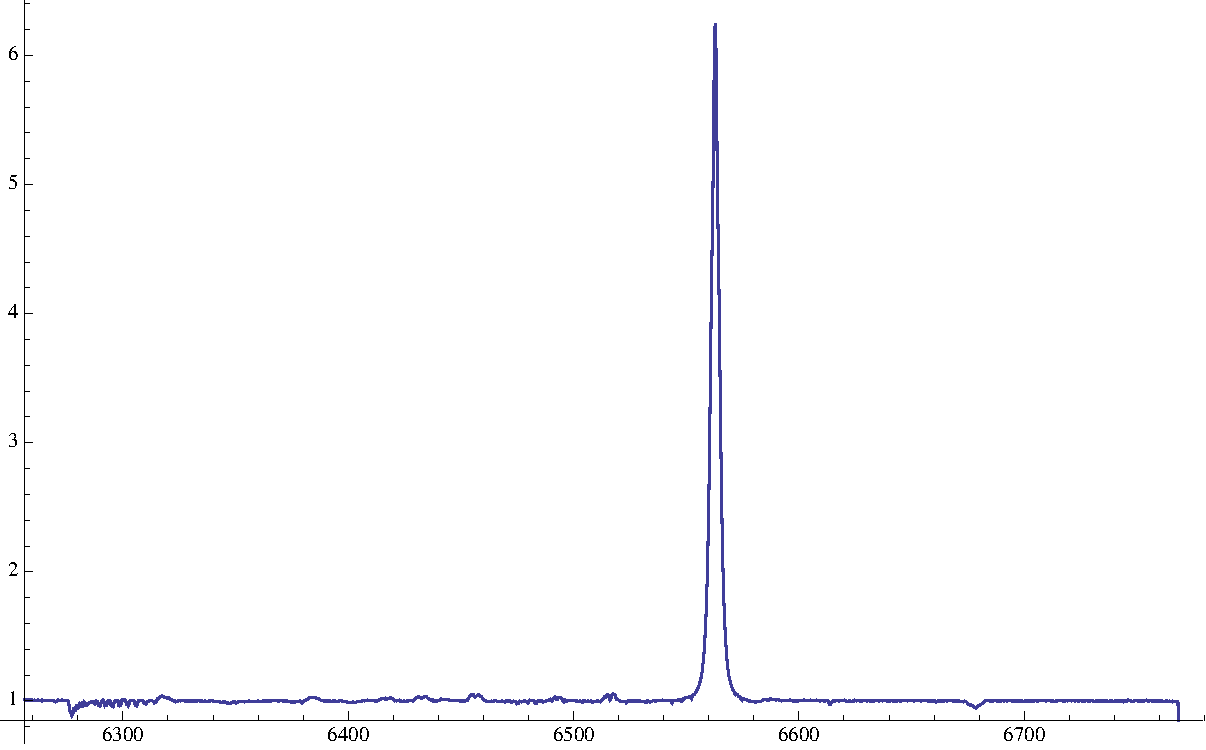
\includegraphics[width=180pt]{emission_spectrum}
\label{fig:pure_emission}
\quad
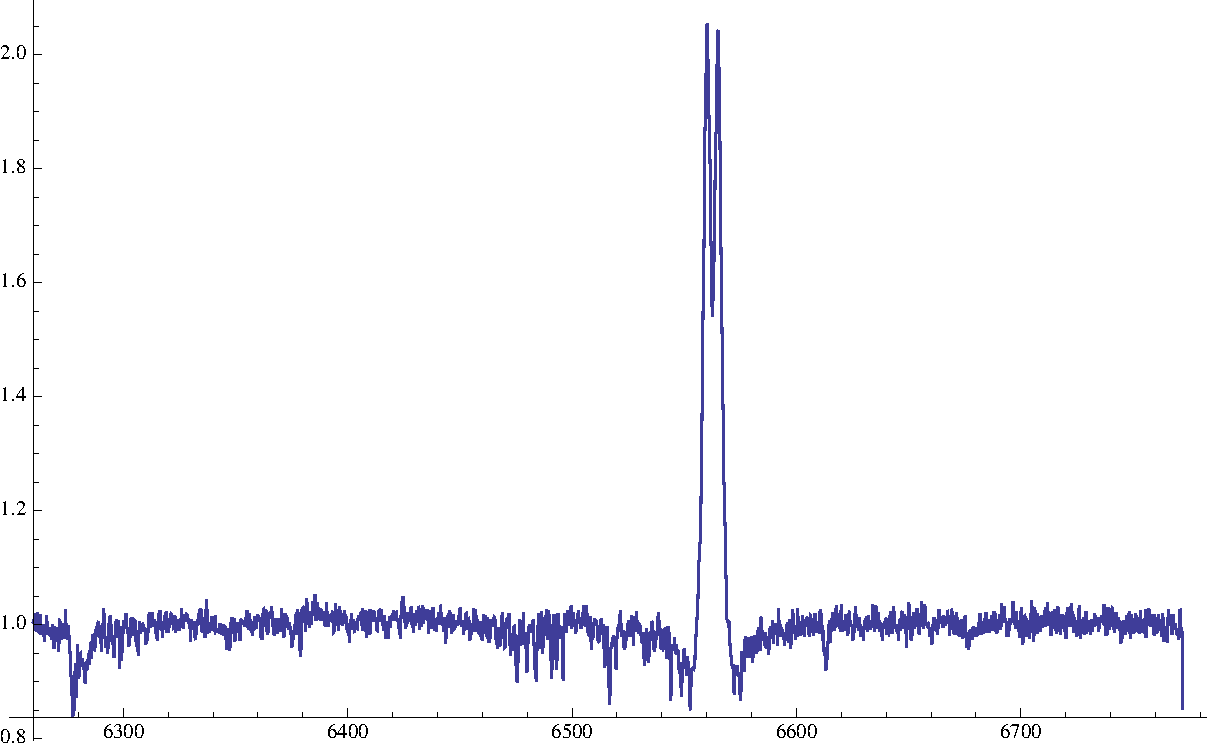
\includegraphics[width=180pt]{small_abs_spectrum}
\caption[Examples of spectra containing pure emission and an emission with an absorption]{Examples of spectra with pure emission (left) and an emission with an absorption(right)}
\label{fig:small_abs}
\end{figure}
\begin{figure}
\centering
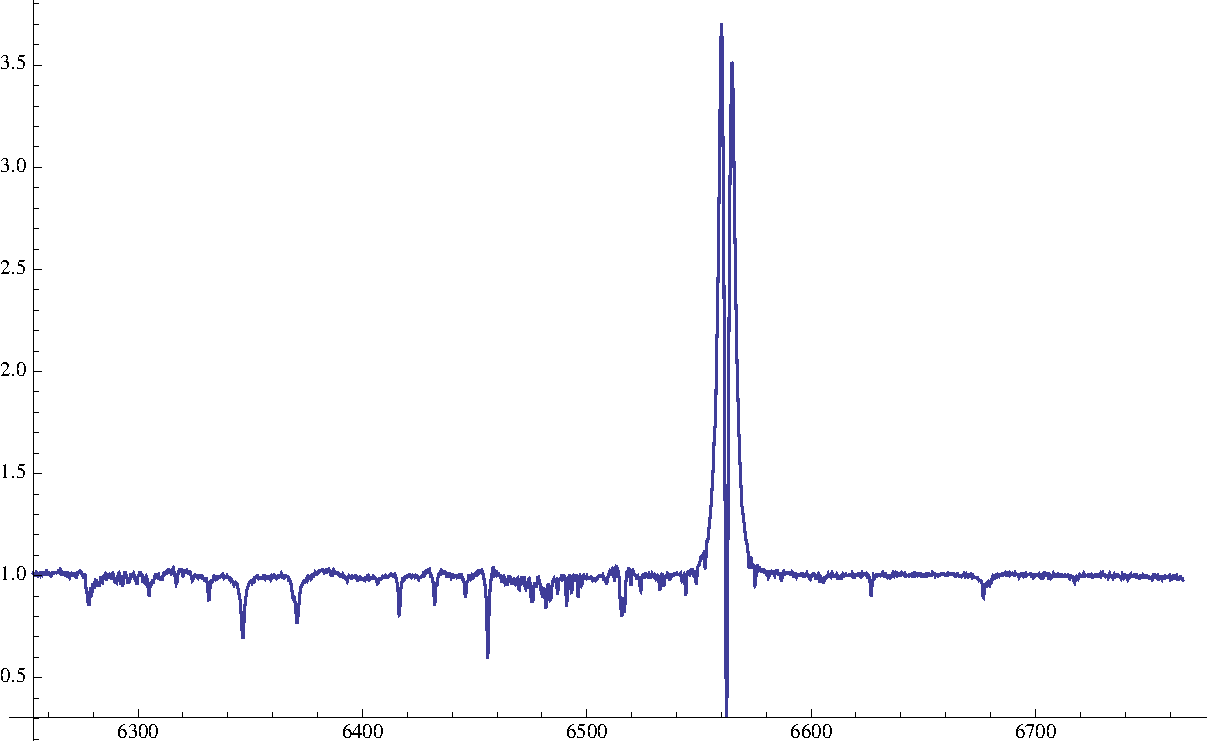
\includegraphics[width=180pt]{big_abs_spectrum}
\label{fig:large_abs}
\centering
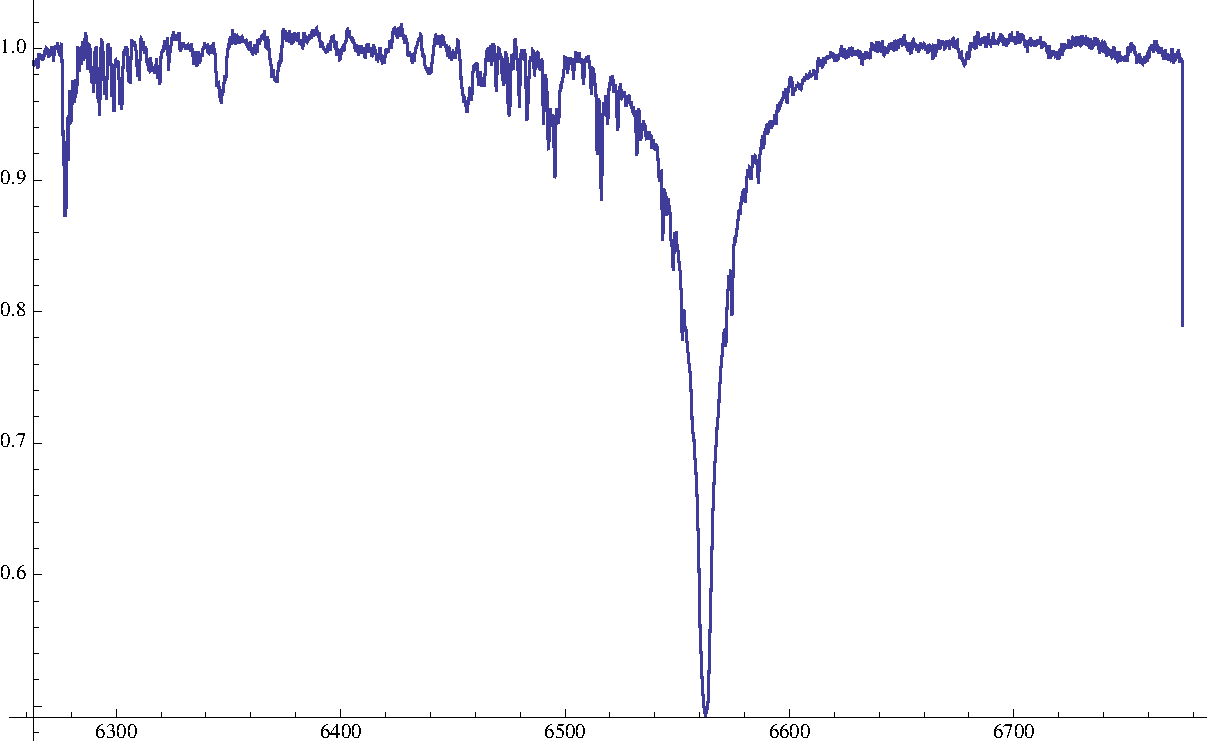
\includegraphics[width=180pt]{absorbtion_spectrum}
\caption[Examples of spectra containing an absorption line with an emission (shell line) and a pure absorption]{Examples of spectra containing an absorption line with an emission (left) and pure absorption (right)}
\label{fig:pure_absrob}
\end{figure}
We provide details of the profiles for the an emission with a central absorption and an absorption line with an emission to illustrate the fine difference between them in Figure~\ref{fig:detail}.
\begin{figure}
\centering
\includegraphics[width=180pt]{big_abs_detail}
\label{fig:large_abs}
\centering
\includegraphics[width=180pt]{small_abs_detail}
\caption[Details of spectra containing an absorption line with an emission (shell line) and an emission with a central absorption]{Details of spectra containing an absorption line with an emission (left) and an emission with a central absorption (right)}
\label{fig:detail}
\end{figure}

We first explored the performance on data extracted from the FITS files that were provided by the Ond{\v r}ejov observatory. Although they do not represent the raw spectra as they were measured, because they had undergone continuum normalization when they were retrieved from the database, we will refer to them as raw data, because we have not done any preprocessing on them specifically for this test. The original data set consists of 1593 FITS files, each containing a binary table with measured values. These values come in a tuple \((\textit{wavelength}, \textit{intensity})\), which represents an intensity of emission at a certain wavelength. In addition to the three types we mentioned, the data set also contains non-Be stars, that have pure absorption (Figure~\ref{fig:pure_absrob}). We've converted these FITS files into one CSV file, that can be imported into machine learning frameworks. We did not do any data transformations and preprocessing, besides the conversion. The data set has 1997 input features, most of them are however irrelevant for the classification, as they either contain noise or values that do not create the characteristic shapes. The data set has 1594 rows, but we had to split it into separate training and testing data sets with two thirds of the rows going into the new training set and the rest into the testing set. We have also excluded the out-of-bag score and the x-validation for the cudaTree implementation for reasons described in section~\ref{sub:wrapper_test}.
\begin{table}[h]
\begin{tabular}{|l|l|l|l|l|}
\hline
trees        & out-of-bag & x-validation & train-test set & time \\ \hline
1            &88.95 \%            &87.82 \%              &91.06 \%                 & 1.1        \\ \hline
10           &91.35 \%            &93.34 \%              &96.00 \%                 & 11       \\ \hline
50           &94.10 \%            &93.72 \%              &95.06 \%                 & 36.43      \\ \hline
100          &94.10 \%            &93.81 \%              &95.24 \%                 & 85.41      \\ \hline
500          &94.28 \%            &93.91 \%              &95.06 \%                 & 428.23     \\ \hline
1000         &94.19 \%            &94.01 \%              &95.06 \%                 & 781        \\ \hline
2000         &94.18 \%            &94.10 \%              &94.67 \%                 & 1456       \\ \hline
\end{tabular}
\caption{Performance of H2O implementation on raw data}
\label{tab:h2o-raw}
\end{table}
\begin{table}[h]
\begin{tabular}{|l|l|l|l|l|}
\hline
trees/values & out-of-bag & x-validation & train-test set & time \\ \hline
1            &40.40 \%           &88.67 \%              &90.11 \%                & 2.04          \\ \hline
10           &90.72 \%           &94.18 \%              &94.87 \%                &2.52           \\ \hline
50           &94.38 \%           &94.65 \%              &94.87 \%                &3.86        \\ \hline
100          &93.91 \%           &94.38 \%              &94.68 \%                &5.95        \\ \hline
500          &93.81 \%           &93.91 \%              &94.87 \%                &21.45      \\ \hline
1000         &94.10 \%           &94.19 \%              &94.87 \%                &38.19         \\ \hline
2000         &94.19 \%           &93.91 \%              &95.25 \%                &74.65        \\ \hline
\end{tabular}
\caption{Performance of scikit implementation on raw data}
\label{tab:scikit-raw}
\end{table}
\begin{table}[h]
\begin{tabular}{|l|l|l|l|l|}
\hline
trees/values & train-test set & time \\ \hline
1            & 11.40 \%              & 3.03      \\ \hline
10           & 94.48 \%              & 3.56      \\ \hline
50           & 94.48 \%              & 3.98      \\ \hline
100          & 95.81 \%              & 4.46      \\ \hline
500          & 94.48 \%              & 7.78     \\ \hline
1000         & 95.43 \%              & 15.97     \\ \hline
2000         & 95.43 \%              & 30.20     \\ \hline
\end{tabular}
\caption{Performance of cudaTree implementation on raw data}
\label{tab:cuda-raw}
\end{table}

\begin{table}[h]
\begin{tabular}{|l|l|l|l|l|l|}
\hline
actual/predicted & 1 & 2 & 3 & 4 & recall \\ \hline
1 & 46 & 12 & 0 & 0 & 0,79 \\ \hline
2 & 5 & 24 & 2 & 0 & 0,78 \\ \hline
3 & 0 & 0 & 384 & 0 & 1.0 \\ \hline
4 & 0 & 8 & 9 & 6 & 0.26 \\ \hline
precision & 0.90 & 0.55 & 0.97 & 1.0 &  \\ \hline
\end{tabular}
\caption{The confusion matrix for a forest of size 2000 on raw data}
\label{tab:confrawdata}
\end{table}
The measured values show, that Random Forest started predicting the data with a good precision early on. We also see, that beyond a certain point, the accuracy stops increasing and reaches a certain limiting value. The model managed to recognize important features, that shape the spectrum, even though they were not consistent through all the data. However, as we see in the confusion matrix in table~\ref{tab:confrawdata}, the forest had problems to successfully recognize members of the fourth category, the spectra that contain absorption line with emission. It classified only a small fraction of them correctly, most of them considering to be either pure absorption or an emission with central absorption. Note, that even though H2O gave very similar results to the other implementations in terms of accuracy, it took significantly longer time to train the model than the rest. This may be due to more complex architecture and generally more inefficient implementation on a single computer, because the framework was intended to run on a distributed cloud. 

Next we examine the performance of Random Forests on data, that have been binned (by the process described in section~\ref{sec:binning}). This aligns the data, making the feature columns more consistent, because they now correspond to the exactly the same wavelength. As we predicted, this increased the accuracy a little. It also decreased the time necessary to train the models.

\begin{table}[h]
\begin{tabular}{|l|l|l|l|l|}
\hline
trees        & out-of-bag & x-validation & train-test set & time \\ \hline
1            &93.51 \%            &91.32 \%              &92.39 \%                 & 3.91        \\ \hline
10           &95.78 \%            &93.34 \%              &97.34   \%                 & 5.74       \\ \hline
50           &97.52 \%            &97.01 \%              &97.56 \%                 & 42.04      \\ \hline
100          &97.75 \%            &97.83 \%              &98.09 \%                 & 85.59      \\ \hline
500          &98.21 \%            &98.12 \%              &98.09 \%                 & 468.53    \\ \hline
1000         &98.31 \%            &98.15 \%               &97.90 \%                 & 851.97        \\ \hline
2000         &98.31 \%            &98.06 \%              &97.71 \%                 & 1656.87       \\ \hline
\end{tabular}
\caption{Performance of H2O implementation on binned data}
\label{tab:h2o-binned}
\end{table}
\begin{table}[h]
\begin{tabular}{|l|l|l|l|l|}
\hline
trees/values & out-of-bag & x-validation & train-test set & time \\ \hline
1            &42.83 \%           &93.99 \%              &93.34 \%                & 2.04          \\ \hline
10           &95.50 \%           &97.85 \%              &97.53 \%                &2.50           \\ \hline
50           &98.41 \%           &98.22 \%              &97.72 \%                &3.88        \\ \hline
100          &98.69 \%           &98.13 \%              &97.91 \%                &5.53        \\ \hline
500          &98.41 \%           &98.22 \%              &97.71 \%                &19.83      \\ \hline
1000         &98.31 \%           &98.31 \%              &97.71 \%                &35.63         \\ \hline
2000         &94.19 \%           &93.91 \%              &97.71 \%                &73.61        \\ \hline
\end{tabular}
\caption{Performance of scikit implementation on binned data}
\label{tab:scikit-binned}
\end{table}
\begin{table}[h]
\begin{tabular}{|l|l|l|l|}
\hline
trees/values & train-test set & time\\ \hline
1&11.22    \%&3.2\\ \hline
10&97.34   \%&3.5\\ \hline
50&96.96   \%&3.9\\ \hline
100&97.15  \%&4.1\\ \hline
500&97.34  \%&7.1\\ \hline
1000&97.34 \%&13.44\\ \hline
2000&97.34 \%&25,33\\ \hline 
\end{tabular}
\caption{Performance of cudaTree implementation on binned data}
\label{tab:cuda-binned}
\end{table}
\begin{table}[h]
\begin{tabular}{|l|l|l|l|l|l|}
\hline
actual/predicted & 1 & 2 & 3 & 4 & recall \\ \hline
1 & 52 & 7 & 0 & 0 & 0,79 \\ \hline
2 & 5 & 63 & 0 & 0 & 0,92 \\ \hline
3 & 0 & 0 & 384 & 0 & 1.0 \\ \hline
4 & 0 & 0 & 0 & 15 & 1.0 \\ \hline
precision & 0.91 & 0.9 & 1.0 & 1.0 &  \\ \hline
\end{tabular}
\caption{The confusion matrix for a forest of size 2000 on binned data}
\label{tab:confbinned}
\end{table}
For the final test, we examined the performance of random forests on data that had undergone feature extraction \cite{bromovabeclass}. This feature extraction consists of centering the data, applying the wavelet transform and an aggregation function. This greatly reduced the dimensionality of the data (in this case, it was from 1997 features to 10) and increased the accuracy of the classification. We see that the forest now correctly recognized most of the data and only confused some of the pure emission spectra with spectra containing central absorption and vice-versa. The reduction in dimensionality significantly improved the speed of the training.
\begin{table}[h]
\begin{tabular}{|l|l|l|l|l|}
\hline
trees        & out-of-bag & x-validation & train-test set & time \\ \hline
1&96.14    \%&95.99 \%&95.28 \%&1.06\\ \hline
10&95.91   \%&97.33 \%&96.23 \%&1.04\\ \hline
50&97.03   \%&97.81 \%&96.23 \%&1.03\\ \hline
100&97.77  \%&98.00 \%&97.17 \%&1.05\\ \hline
500&97.98  \%&98.09 \%&98.11 \%&2.10\\ \hline 
1000&97.98 \%&98.19 \%&98.11 \%&4.16\\ \hline
2000&98.09 \%&98.19 \%&98.11 \%&8.40\\ \hline
\end{tabular}
\caption{Performance of H2O implementation on extracted features}
\label{tab:h2o-extracted}
\end{table}
\begin{table}[h]
\begin{tabular}{|l|l|l|l|l|}
\hline
trees/values & out-of-bag & x-validation & train-test set & time \\ \hline
1&41.98    \%&96.76 \%&96.32 \%&0.01\\ \hline
10&96.85   \%&98.09 \%&97.87 \%&0.11\\ \hline
50&98.38   \%&98.28 \%&98.07 \%&0.15\\ \hline 
100&98.47  \%&98.47 \%&98.26 \%&0.24\\ \hline
500&98.57  \%&98.76 \%&97.87 \%&0.99\\ \hline
1000&98.57 \%&98.57 \%&98.26 \%&1.92\\ \hline
2000&98.66 \%&98.57 \%&98.26 \%&3.74\\ \hline
\end{tabular}
\caption{Performance of scikit implementation on extracted features}
\label{tab:scikit-extracted}
\end{table}
\begin{table}[h]
\begin{tabular}{|l|l|l|}
\hline
trees/values & train-test set & time \\ \hline
1&10.25    \%&0.05\\ \hline
10&98.07   \%&0.18\\ \hline
50&98.65   \%&0.60\\ \hline
100&99.03  \%&1.13\\ \hline
500&99.03  \%&5.37\\ \hline
1000&98.65 \%&7.48\\ \hline
2000&99.03 \%&15.3\\ \hline 
\end{tabular}
\caption{Performance of cudaTree implementation on extracted features}
\label{tab:cuda-extracted}
\end{table}
\begin{table}[h]
\begin{tabular}{|l|l|l|l|l|l|}
\hline
actual/predicted & 1 & 2 & 3 & 4 & recall \\ \hline
1 & 51 & 2 & 0 & 0 & 0.96 \\ \hline
2 & 2 & 63 & 2 & 0 & 0.94 \\ \hline
3 & 0 & 0 & 381 & 0 & 1.0 \\ \hline
4 & 0 & 0 & 2 & 14 & 1.0 \\ \hline
precision & 0.96 & 0.97 & 0.99 & 1.0 &  \\ \hline
\end{tabular}
\caption{The confusion matrix for a forest of size 2000 on extracted features}
\label{tab:confextra}
\end{table}
For comparison, in table~\ref{tab:spectra_allml} we provide performance of several other machine learning algorithms on these data. We also include the best score of Random Forests for each data set.
\begin{table}
    \begin{tabular}{|l|l|l|l|l|}
    \hline
    ~              & RDF       & DL       & SVM      & kNN      \\ \hline
    Raw Data       & 96.00 \%  & 93.16 \%   & 75.39 \% & 93.73 \% \\ \hline
    Binned Data    & 97.71 \%  & 98.10 \%   & 85.36 \% & 96.96 \% \\ \hline
    Extracted Data & 99.03 \%  & 98,87 \% & 95.83 \% & 95.74 \% \\ \hline
    \end{tabular}
    \caption{Comparison of several machine learning algorithms on the data}
    \label{tab:spectra_allml}
\end{table}

\subsection{Redshift prediction}
Redshift is a phenomenon that happens when an electromagnetic radiation of an object increases its wavelength. In this case we are dealing with a cosmological redshift, which determines how quickly galaxies move from each other and according to the Hubble's law \cite{hubble1937observational}, also determines how far they are from each other. This is used mainly do determine their distance and relative position to us. Redshifts can be accurately measured by spectroscopy, however these measurements take a lot of time and because of that, there is only a small amount of measurements. On the other hand, photometry takes much less time to take, however it doesn't provide results that are as accurate as spectroscopic. There is however a relationship between color indices measured by photometry and the redshifts of space objects. Machine learning attempts to model these relationships and predict redshifts form them. 

The data set consists of 4 input attributes and an output continuous attribute. It was taken from a Sloan Digital Sky Survey (SDSS) and contains spectroscopic redshifts along with photometric color indices. The four features are differences between the color bands of ultraviolet, green, red and infrared and their redshift, while the output contains redshifts. The prediction in this case is a predicted photometric redshift based on the colors.
\begin{table}[h]
\begin{tabular}{|l|l|l|l|l|}
\hline
trees/values & out-of-bag & train-test set & time \\ \hline
1            &89.91 \%                   &87.32 \%                & 0.41          \\ \hline
10           &88.37\%                    &92.81 \%                &1.30           \\ \hline
50           &92.93 \%                   &92.97 \%                &5.25        \\ \hline
100          &92.97 \%                   &93.20 \%                &10.03        \\ \hline
500          &93.13 \%                   &93.30 \%                &46.64      \\ \hline
1000         &93.17 \%                   &93.23 \%                &93.46         \\ \hline
2000         &92.96 \%                   &93.43 \%                &185.10        \\ \hline
\end{tabular}
\caption{Performance of scikit implementation on redshift prediction}
\label{tab:scikit-redshift}
\end{table}
\section{Common machine learning data sets}
We have conducted experiments on these data sets from the UCI repository \cite{uci} : ISOLET\footnote{\url{https://archive.ics.uci.edu/ml/datasets/ISOLET}}, Adult\footnote{\url{http://archive.ics.uci.edu/ml/datasets/Adult}}, Internet Advertisements \footnote{\url{http://archive.ics.uci.edu/ml/datasets/Internet+Advertisements}}. We have chosen these data sets either for their high dimensionality, lots of samples, or both. We include a table with best results on each data set. We have tested them with Random Forest, Deep Learning, kNN and Support Vector Machine. 
\begin{table}[h]
    \begin{tabular}{|l|l|l|l|l|}
    \hline
    ~      & RDF      & DLNN     & SVM     & kNN     \\ \hline
    ISOLET & 94.80 \% & 92.05 \% & 85.4 \% & 91.34 \%   \\ \hline
    Adult  & 86.41 \% & 88.14 \% & 75.14 \%  & 72.64 \%  \\ \hline
    Ads    & 98.65 \% & 96.27 \% & 85.01\% & 94.09 \% \\ \hline
    \end{tabular}
    \caption{Performance comparison on UCI data sets}
\end{table}
\section{Experiment outcome and conclusion}
From the measured values on all three experiments we see, that the GPU implementation significantly decreased the time of the induction, in some cases the speedup was more than three times compared to the time of the induction by the scikit implementation, without decreasing the accuracy of the forest. However for the data with the extracted features, the GPU took longer to grow the forest than both H2O and scikit. This may be due to the overhead the use of GPUs introduces, as explained in Section \ref{sec:rdf_gpu}. We also see, that in the tests on the raw and the binned data, the H2O had significantly worse time than both scikit and cudaTree. However we expect that in case of a huge amount of spectra, its ability to distribute data across several computing nodes and build forests in a MapReduce environment would be necessary, because neither scikit nor cudaTree are capable of distributed computing. Based on this, we recommend using scikit when you do not have to use a cloud environment and only resort to H2O when you need to process large data sets.

When compared with other machine learning algorithms, the Random Forests outperformed other algorithms in accuracy on both raw data and on extracted features. They were beaten only by the Deep Learning neural network on binned data. We however did not try to optimize the parameters of the other algorithms much, so it is very much possible their results could improve a bit. 
\setsecnumdepth{part}
\chapter{Conclusion}
We have examined the machine learning model Random Decision Forest and its performance on astronomical data and large data sets. We include a description of an algorithm of Random Forest that runs on a MapReduce model and is able to scale for very large data sets. We also provide a survey of implementations that run on a GPGPU platform.

We also implemented a Python package, that wraps several implementations of Random Forests and allows to train and test models with a run of a single executable file. This implementation was tested on astronomical data, as well as some larger data sets from the UCI repository. The RDF model has shown that it is capable of precise classification and regression of data. We have found, that on small data even smaller forests will do, however when the size of the data increases, we need to use larger ensemble. Since the time of induction of a tree is dependent on both size of the data set as well as on the number of the features and the training time of a forest is linearly dependent on the number of trees, training on bigger data becomes quickly unfeasible. This calls for a efficient distributed implementation.

 We will integrate the wrapper presented in this thesis in a cloud environment in Ond{\v r}ejov observatory, so others can build models from their data. For the future work, we would like to develop an efficient, scalable, massively parallel implementation of the algorithm that could run on several computing nodes, since most of today's publicly available implementations are not meant to analyze Big Data. The results have been presented at an international conference called \emph{New challenges in astro- and environmental informatics in the Big Data era}\footnote{\url{https://bigdataconf.gothard.hu/indico/conferenceDisplay.py?confId=1}}.
\bibliographystyle{iso690}
\bibliography{bibliography}

\setsecnumdepth{all}
\appendix

\chapter{Acronyms}
% \printglossaries
\begin{description}
	\item[RDF] Random decision forest
	\item[RF] Random forest
	\item[DT] Decision tree
	\item[SPDT] Streaming Parallel Decision Tree
	\item[DL] Deep Learning
	\item [DL] Deep Learning Neural Network
	\item [SVM] Support Vector Machine
	\item [kNN] k-Nearest Neighbors
\end{description}

\chapter{Wrapper usage documentation and file format}
The wrapper depends on following Python packages:
\begin{itemize}
\item scikit-learn
\item numpy
\item requests
\item pandas
\item cudaTree
\end{itemize}
The wrapper is designed to run under Python 3 or higher and does not offer some functionality under lower versions. However, running the cudaTree package is supported only under Python 2.7, due to the technical limitations of the library. To run H2O, the user have to have Java installed. The H2O instance can run prior to the execution of the wrapper, or if there is no instance running, the wrapper will start it provided it finds an h2o.jar file in the root folder of the wrapper. The wrapper is run by running the command \texttt{python 3 runRF [input\_file1, ...]}, which will run it in Python 3. For Python 2, just change the initial command for \texttt{python2}. The wrapper is available on the following git repository for public access:\\\url{https://github.com/palicand/random-forest-wrapper}.

The wrapper requires at least one JSON files as an argument on the command line. It does not accept any other arguments or configuration files. The wrapper considers each input file as a discrete experiment. We provide an example of the input file and descriptions of its parameters.
\begin{description}
\item[name] a name of the experiment, several output files created for the experiment are named according to this option
\item[trees] a number of trees
\item[implementation] implementation to use, can be scikit or h2o
\item[min\_split] minimal amount of classes in a node for it to be eligible for split
\item[depth] maximal depth of the tree
\item[mode] classification, regression or gpu
\item[splitting\_criterion] ENTROPY or GINI
\item[features] number of features to consider in each tree, can be an integer of ``auto''. If ``auto'', the wrapper will use sqrt(n\_features) in as the number of features to consider.
\item[sample\_ratio]: a ratio by with to do bagging
\item[bin\_limit]: how many bins for the histograms to create, only valid for H2O
\item[seed]: the initial seed for the random number generator
\item[parallel]: if the algorithm should run in parallel, can be 1 or 0
\item[error\_estimate]: if we want the error estimate
\item[ignore]: a list of features to ignore, can be the name of the feature, if the header was provided or its index
\item[label]: which column contains the label, see above for possible values
\item[sampling]: what sampling to use, can be RANDOM or STRATIFIED
\item[run\_test]: if you want to do scoring test
\item[create\_test\_set]: if you want to create test set
\item[test\_set\_ratio]: what ratio to use when creating test set
\item[compute\_f1]: if you want to compute f1 score
\item[compute\_cf]: if you want to compute confusion matrix
\item[data\_sets]: must contain train\_set, can contain score\_set and prediction\_set
\item[path] the path to the data set
\item[file\_type] can be fits or CSV
\item[delimiter] if CSV, this is the delimiter
\item[header] if the file contains header
\item[binning] if fits, perform binning
\item[cross\_validation] if present, the wrapper will perform cross-validation, folds determines the number of folds
\end{description}
\begin{lstlisting}
{
	"name":"spectra_binned",
	"trees": 2000,
	"implementation":"scikit",
	"min_split": 4,
	"mode": "classification",
	"splitting_criterion": "ENTROPY",
	"features": 44,
	"depth":2147483647,
	"sample_ratio":67,
	"bin_limit":1600,
	"seed":5364668453,
	"parallel":1,
	"error_estimate":1,
	"ignore":["id"],
	"label":"class",
	"sampling":"RANDOM",
	"run_test": true,
	"create_test_set":false,
	"test_set_ratio":0.67,
	"compute_f1": true,
	"compute_cf": true,
	"data_sets":
	{
		"train_set": 
		{
			"path": "processed_spectra_train.csv",
			"file_type": "csv",
			"delimiter": ",",
			"header": true,
			"binning":false
		},
		"score_set": 
		{
			"path": "processed_spectra_test.csv",
			"file_type": "csv",
			"delimiter": ",",
			"header": true

		}
	},
	"cross_validation":
	{
		"folds": 10
	}
}
\end{lstlisting}
The wrapper will write its output to a file named \texttt{result.json}. Its root object contains an array of objects, each named after an input file the wrapper received at its command line. An example of the output file is provided below:
\begin{lstlisting}
{
	"scikit_extracted_2000.json": 
	{
		"training_oob_scores": [[2000, 
			0.9875954198473282]], 
		"score": [["extracted_test.csv", 
			2000, 0.9845261121856866]],
		"training_time": [[2000, 4.452026]], 
	 	"f1_score": [[0.9622641509433962, 
	 		0.9545454545454547, 0.9947780678851175, 
	 		0.9333333333333333]], 
		"xvalidation_precision": [[2000, 
			0.9809957445009652]], 
	 	"conf_matrix": [[[51, 2, 0, 0], 
	 		[2, 63, 2, 0], [0, 0, 381, 0], [0, 0, 2, 14]]]
	 }
}
\end{lstlisting}
\chapter{Contents of enclosed CD}


%change appropriately

\begin{figure}
	\dirtree{%
		.1 readme.txt\DTcomment{the file with CD contents description}.
		.1 src\DTcomment{the directory of source codes}.
		.2 wrapper\DTcomment{wrapper sources}.
		.2 thesis\DTcomment{the directory of \LaTeX{} source codes of the thesis}.
		.1 text\DTcomment{the thesis text directory}.
		.2 thesis.pdf\DTcomment{the thesis text in PDF format}.
	}
\end{figure}

\end{document}
